\documentclass[11pt]{article}

\usepackage[margin=1in]{geometry}
\usepackage{amsmath,amssymb,amsthm,mathtools}
\usepackage{booktabs}
\usepackage{enumitem}
\usepackage{xcolor}
\usepackage{microtype}
\usepackage{tikz}
\usetikzlibrary{arrows.meta,positioning,calc}
\usepackage[colorlinks=true,linkcolor=blue!50!black,citecolor=green!40!black,urlcolor=blue!60!black]{hyperref}

% --- operators ---
\DeclareMathOperator{\Tr}{Tr}
\DeclareMathOperator{\vecop}{vec}
\DeclareMathOperator{\Var}{Var}
\DeclareMathOperator{\rank}{rank}
\DeclareMathOperator{\diag}{diag}
\DeclareMathOperator{\Hom}{Hom}
\DeclareMathOperator{\im}{im}
\DeclareMathOperator*{\argmin}{arg\,min}
\newcommand{\HH}{\mathcal{H}}
\newcommand{\KK}{\mathcal{K}}
\newcommand{\LL}{\mathcal{L}}
\newcommand{\R}{\mathbb{R}}
\newcommand{\C}{\mathbb{C}}
\newcommand{\Z}{\mathbb{Z}}
\newcommand{\ket}[1]{\lvert #1 \rangle}
\newcommand{\bra}[1]{\langle #1 \rvert}
\newcommand{\braket}[2]{\langle #1 \vert #2 \rangle}
\newcommand{\inner}[2]{\langle #1, #2 \rangle}
\newcommand{\norm}[1]{\lVert #1 \rVert}
\newcommand{\abs}[1]{\lvert #1 \rvert}
\newcommand{\bd}{\partial}
\newcommand{\dd}{\mathrm{d}}

\theoremstyle{definition}
\newtheorem{definition}{Definition}[section]
\newtheorem{remark}[definition]{Remark}
\newtheorem{example}[definition]{Example}
\theoremstyle{plain}
\newtheorem{theorem}[definition]{Theorem}
\newtheorem{proposition}[definition]{Proposition}
\newtheorem{lemma}[definition]{Lemma}
\newtheorem{corollary}[definition]{Corollary}

% honest-caveat callout
\newcommand{\caveat}[1]{\par\noindent\textcolor{red!60!black}{\textbf{Caveat.}}\ #1\par}

\title{\bfseries Bulk Cobordism Synthesis by\\ Entanglement-Sourced Regge Sampling\\[4pt]
\large Theory and Implementation Plan}
\author{Andrew Kelleher}
\date{}

\begin{document}
\maketitle

\begin{abstract}
\noindent
We develop the theory of, and an implementation plan for, a single construction:
given a quantum operation $U:\HH_B\to\HH_A$ between two boundary systems, \emph{synthesize a
bulk geometry} that realizes it. The bulk is a simplicial complex whose metric is the
mutual information between quantum subsystems, whose dynamics is the discrete
gravitational (Regge) action, and whose boundary is held \emph{fixed} while the interior
is rewritten by Monte Carlo moves. Realizability is the statement that a prescribed
boundary state can be made a harmonic mode of the bulk Laplacian; we minimize the
corresponding residual while holding the boundary fixed. The document is written as a
sequence of self-contained tutorials on each mathematical object (mutual information and
the information metric, simplicial complexes, the Choi--Jamio\l{}kowski isomorphism, the
Hodge Laplacian, the Regge action, Pachner moves, the heat-kernel spectral dimension),
followed by the synthesis theory (the gravitational posterior, feasibility witnesses, and
the free-energy certificate of obstruction) and a concrete implementation plan against the
existing codebase. The emphasis throughout is theoretical. Honest scope statements,
prior-art positioning (the mutual-information metric is due to Cao--Carroll--Michalakis),
and the evidentiary bar for any emergent-dimension claim are stated explicitly.
\end{abstract}

\tableofcontents

% ======================================================================
\section{Overview}
\label{sec:overview}

\subsection{The problem}

A topological quantum field theory assigns, to each boundary surface $\Sigma$, a Hilbert
space $Z(\Sigma)$, and to each bulk $W$ with $\bd W = \Sigma$ a vector $Z(W)\in
Z(\Sigma)$. A morphism between two boundaries $A,B$ is, in this language, a cobordism: a
bulk $W_{AB}$ interpolating between them. The inverse question is the subject of this
document:

\begin{quote}
\itshape Given an operation $U:\HH_B\to\HH_A$ relating two boundary systems, construct a
bulk $W_{AB}$ that realizes it --- rather than assuming one is given.
\end{quote}

Our strategy is to make ``realizes'' precise and computable. We bend $U$ into a boundary
\emph{state} $\psi_U$ (Choi--Jamio\l{}kowski), build a discrete bulk whose geometry is
sourced by quantum entanglement, and demand that $\psi_U$ be a harmonic (zero) mode of the
bulk's Hodge Laplacian on the prescribed, fixed boundary. The degree to which this can be
achieved is measured by a residual $r$; the central computational task is

\begin{equation}
\boxed{\;\text{minimize the residual } r \text{ while holding the boundary fixed.}\;}
\label{eq:goal}
\end{equation}

\subsection{The construction in one equation}

All of the theory below is organized around a single probability measure on bulk geometries
$K$ whose boundary subcomplex $L=\bd K$ is held fixed:
\begin{equation}
\pi_{\tau,\beta}(K)\;\propto\;
\exp\!\Big[\,-\beta\,S_{\mathrm{Regge}}(K)\;-\;\tfrac{1}{\tau}\,r_U(K)\,\Big],
\qquad K\big|_{\bd}=L .
\label{eq:posterior}
\end{equation}
Here $S_{\mathrm{Regge}}$ is the discrete Einstein--Hilbert action (a \emph{gravitational
prior} on geometries), $r_U(K)$ is the realizability residual (a \emph{likelihood} that the
geometry carries the operation $U$), $\beta$ is the gravitational inverse temperature, and
$\tau\downarrow 0$ sharpens the measure onto realizing geometries. Sampling
\eqref{eq:posterior} by Markov chain Monte Carlo, with moves that never touch the fixed
boundary, is the synthesis algorithm. Each symbol is defined and motivated in its own
tutorial section below; the synthesis theory (Section~\ref{sec:synthesis}) explains why this
particular measure is the right object and what its samples certify.

\subsection{Map of the document}

Section~\ref{sec:prelim} is the tutorial core: a self-contained pass over every
mathematical element. Section~\ref{sec:synthesis} assembles them into the synthesis theory.
Section~\ref{sec:impl} is the implementation plan against the existing code.
Section~\ref{sec:assessment} states the honest novelty and 4D-evidence positions. A reader
who only wants the theory can stop after Section~\ref{sec:synthesis}.

\begin{figure}[t]
\centering
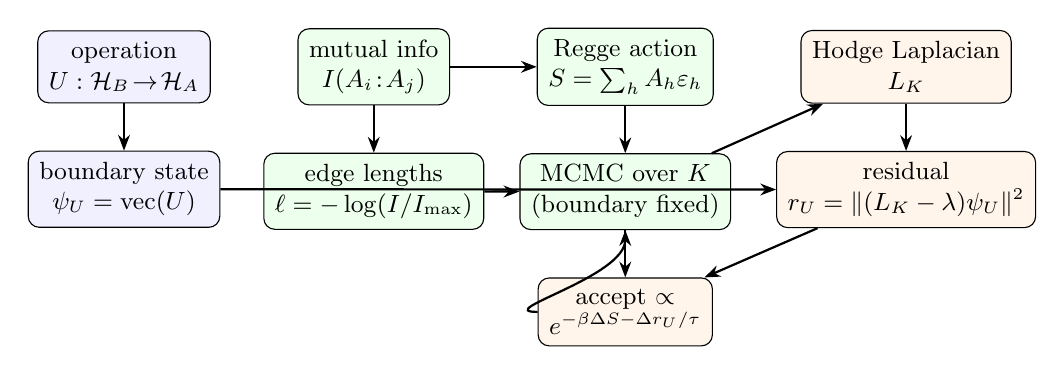
\begin{tikzpicture}[
  node distance=6mm and 11mm,
  box/.style={draw, rounded corners, align=center, inner sep=4pt, font=\small, minimum height=8mm},
  op/.style={box, fill=blue!6},
  geo/.style={box, fill=green!7},
  outp/.style={box, fill=orange!8},
  arr/.style={-{Stealth[length=2mm]}, thick}
]
\node[op] (U) {operation\\$U:\HH_B\!\to\!\HH_A$};
\node[op, below=of U] (psi) {boundary state\\$\psi_U=\vecop(U)$};
\node[geo, right=of U] (mi) {mutual info\\$I(A_i\!:\!A_j)$};
\node[geo, below=of mi] (len) {edge lengths\\$\ell=-\log(I/I_{\max})$};
\node[geo, right=of mi] (regge) {Regge action\\$S=\sum_h A_h\varepsilon_h$};
\node[geo, below=of regge] (mc) {MCMC over $K$\\(boundary fixed)};
\node[outp,right=of regge] (L) {Hodge Laplacian\\$L_K$};
\node[outp,below=of L] (r) {residual\\$r_U=\norm{(L_K-\lambda)\psi_U}^2$};
\node[outp,below=of mc] (acc) {accept $\propto$\\$e^{-\beta\Delta S-\Delta r_U/\tau}$};

\draw[arr] (U) -- (psi);
\draw[arr] (mi) -- (len);
\draw[arr] (len) -- (mc);
\draw[arr] (mi) -- (regge);
\draw[arr] (regge) -- (mc);
\draw[arr] (mc) -- (L);
\draw[arr] (L) -- (r);
\draw[arr] (psi) -- (r);
\draw[arr] (r) -- (acc);
\draw[arr] (mc) -- (acc);
\draw[arr] (acc.west) to[out=180,in=-90] (mc.south);
\end{tikzpicture}
\caption{The synthesis pipeline. The operation is bent to a boundary state (left). The
quantum subsystems' mutual information sets the simplicial edge lengths and the Regge
action (centre). Monte Carlo rewrites the interior at fixed boundary; each geometry yields
a Hodge Laplacian whose harmonic is compared to $\psi_U$, and the residual feeds back into
the acceptance (right).}
\label{fig:pipeline}
\end{figure}

% ======================================================================
\section{Mathematical preliminaries: a tutorial on each element}
\label{sec:prelim}

This section introduces, from first principles, each object appearing in
\eqref{eq:posterior} and Figure~\ref{fig:pipeline}. Each subsection states a definition,
gives the intuition, names the role the object plays in the construction, and flags the one
caveat that matters.

% ----------------------------------------------------------------------
\subsection{Quantum states, reduced density matrices, partial trace}
\label{sec:qstate}

A quantum system is a complex Hilbert space $\HH$ with a chosen orthonormal basis
$\{\ket{i}\}$. A pure state is a unit vector $\ket{\psi}\in\HH$; a general (possibly mixed)
state is a \emph{density matrix} $\rho$: a positive semidefinite operator with
$\Tr\rho=1$. A pure state corresponds to the rank-one projector $\rho=\ket{\psi}\bra{\psi}$.

For a bipartite system $\HH_{AB}=\HH_A\otimes\HH_B$, the state of subsystem $A$ alone is the
\emph{reduced density matrix}, obtained by the \emph{partial trace} over $B$:
\begin{equation}
\rho_A \;=\; \Tr_B\,\rho_{AB}
\;=\; \sum_{b} (\,\mathbb{1}_A\otimes\bra{b}\,)\,\rho_{AB}\,(\,\mathbb{1}_A\otimes\ket{b}\,).
\end{equation}
The partial trace is the unique operation consistent with the requirement that local
measurements on $A$ are reproduced by $\rho_A$.

\paragraph{Role.} In the construction, the ``quantum subsystems'' are factors of a large
state produced by an interaction history; their reduced density matrices are the raw
material from which entanglement --- and hence geometry --- is computed
(Section~\ref{sec:mi}). In the codebase these are the per-vertex $\rho$ and per-pair joint
$\rho_{AB}$ tracked during the Monte Carlo.

% ----------------------------------------------------------------------
\subsection{Entanglement entropy and mutual information}
\label{sec:mi}

\begin{definition}[von Neumann entropy]
The entropy of a state $\rho$ is $S(\rho) = -\Tr\big(\rho\log\rho\big)
= -\sum_k p_k \log p_k$, where $\{p_k\}$ are the eigenvalues of $\rho$.
\end{definition}

For a \emph{pure} global state, $S(\rho_A)=S(\rho_B)$ quantifies the entanglement between
$A$ and its complement; it vanishes iff the state factorizes ($\ket{\psi}=\ket{\psi_A}\otimes\ket{\psi_B}$).

\begin{definition}[mutual information]
For subsystems $A,B$ the mutual information is
\begin{equation}
I(A:B)\;=\;S(\rho_A)+S(\rho_B)-S(\rho_{AB})\;\ge\;0,
\end{equation}
with equality iff $\rho_{AB}=\rho_A\otimes\rho_B$ (no correlation, classical or quantum).
\end{definition}

Mutual information is the total correlation between two subsystems. It is symmetric,
nonnegative, and --- crucially for what follows --- it is large when subsystems are
strongly correlated and small when they are nearly independent. It upper-bounds all
two-point correlators (a consequence of subadditivity), so ``high mutual information''
literally means ``these two subsystems strongly influence one another.''

\paragraph{Role.} Mutual information is the bridge from quantum dynamics to geometry: two
subsystems that are strongly correlated will be \emph{close} in the emergent metric
(Section~\ref{sec:metric}). This is the Van~Raamsdonk slogan ``entanglement is the glue of
spacetime'' \cite{vanraamsdonk2010} made quantitative.

% ----------------------------------------------------------------------
\subsection{The mutual-information metric}
\label{sec:metric}

We turn correlation into distance. The defining choice is a monotone decreasing map from
mutual information to an edge length: strong correlation $\mapsto$ short edge.

\begin{definition}[information length]
For an edge $e=(i,j)$ between subsystems carrying mutual information $I_{ij}$,
\begin{equation}
\ell_{e} \;=\; -\log\!\Big(\frac{I_{ij}}{I_{\max}}\Big),
\label{eq:milength}
\end{equation}
with $I_{\max}$ a normalization (the maximal attainable mutual information) and a floor
$\ell_e \le -\log\varepsilon$ enforced when $I_{ij}<\varepsilon I_{\max}$.
\end{definition}

As $I_{ij}\to I_{\max}$ the length $\ell_e\to 0$ (maximally correlated subsystems are
coincident); as $I_{ij}\to 0$ the length diverges (uncorrelated subsystems are infinitely
far apart). The squared lengths $\ell_e^2$ are the dynamical variables of the discrete
geometry.

\begin{remark}[prior art --- positioning]
The functional form \eqref{eq:milength} is \emph{not original to this work}. It is exactly
the ansatz of Cao, Carroll, and Michalakis \cite{cao2017}, who take an edge weight
$\propto \Phi(I/I_0)$ with $\Phi(x)=-\log x$ on normalized mutual information, and
reconstruct geometry from it by multidimensional scaling. Any presentation of the present
construction must cite \cite{cao2017} for the metric and locate its own contribution
elsewhere (Section~\ref{sec:assessment}): in the \emph{sampled} Regge dynamics, the
\emph{fixed-boundary} synthesis, and the \emph{inverse} (operation-realizing) direction,
none of which appear in \cite{cao2017}.
\end{remark}

\caveat{Mutual-information distance is not automatically a metric. The triangle inequality
can fail; on $1$D quantum chains it holds only within a window of the correlation-decay
exponent \cite{leighton2025}, and fails in gapped/exponentially-correlated phases. Because
the Regge action below requires non-degenerate simplices (valid triangle inequalities on
each cell), the realized edge lengths \eqref{eq:milength} must be checked for simplicial
validity; the floor $-\log\varepsilon$ mitigates but does not guarantee it.}

% ----------------------------------------------------------------------
\subsection{Simplicial complexes: the discrete bulk}
\label{sec:complex}

\begin{definition}[abstract simplicial complex]
A simplicial complex $K$ on a vertex set $V$ is a collection of finite subsets (simplices)
of $V$, closed under taking subsets. A $k$-simplex has $k+1$ vertices; $0$-simplices are
vertices, $1$-simplices edges, $2$-simplices triangles, $3$-simplices tetrahedra, and a
$4$-simplex has $5$ vertices and $\binom{5}{2}=10$ edges.
\end{definition}

A \emph{geometric} (Regge) simplicial complex additionally assigns a squared length
$\ell_e^2$ to each edge; this is the discrete metric. The codimension-one faces lying in
exactly one top-dimensional simplex form the \emph{boundary} $\bd K$; the rest is the
\emph{interior}. This boundary/interior partition is the structural object we will pin in
\eqref{eq:goal}.

\begin{example}[the interaction bowtie is a $4$-simplex]
In the interaction-history model, a pairwise interaction of systems $X,Y$ produces three
outputs --- the two local marginals $X',Y'$ and a joint hub $AB$ --- and glues in the
$5$-vertex cell $\{X,Y,X',AB,Y'\}$ with all $10$ edges. This is precisely (the $1$-skeleton
of) a $4$-simplex; each interaction contributes one unit of local $4$-volume.
See Figure~\ref{fig:bowtie}.
\end{example}

\begin{figure}[t]
\centering
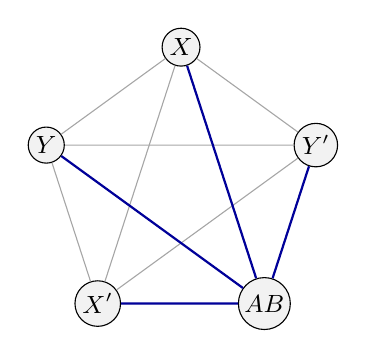
\begin{tikzpicture}[scale=1.5,
  v/.style={circle, draw, fill=black!5, inner sep=1.2pt, font=\small},
  e/.style={gray!70}]
\node[v] (X)  at (90:1.2)  {$X$};
\node[v] (Y)  at (162:1.2) {$Y$};
\node[v] (Xp) at (234:1.2) {$X'$};
\node[v] (AB) at (306:1.2) {$AB$};
\node[v] (Yp) at (18:1.2)  {$Y'$};
\foreach \a/\b in {X/Y,X/Xp,X/AB,X/Yp,Y/Xp,Y/AB,Y/Yp,Xp/AB,Xp/Yp,AB/Yp}
  \draw[e] (\a)--(\b);
% highlight hub spokes
\foreach \a in {X,Y,Xp,Yp} \draw[blue!60!black, thick] (\a)--(AB);
\end{tikzpicture}
\caption{The interaction ``bowtie'': two inputs $X,Y$ produce two local marginals $X',Y'$
and a joint hub $AB$, gluing in a $4$-simplex ($K_5$, ten edges). Hub spokes (blue) carry
the joint mutual information; worldline self-edges carry the input entropies; the three
cross-worldline edges are set to zero mutual information in the local-frame model.}
\label{fig:bowtie}
\end{figure}

% ----------------------------------------------------------------------
\subsection{The Choi--Jamio\l{}kowski isomorphism: bending an operator to a state}
\label{sec:choi}

To ask whether a \emph{geometry} carries an \emph{operation}, we first convert the
operation into a state living on the boundary.

\begin{definition}[vectorization / Choi--Jamio\l{}kowski]
For a linear operator $U:\HH_B\to\HH_A$ with matrix entries $U_{ij}$ in fixed bases, its
vectorization is
\begin{equation}
\psi_U \;=\; \vecop(U)\;=\;\sum_{i,j} U_{ij}\,\ket{i}_A\otimes\ket{j}_B \;\in\; \HH_A\otimes\HH_B .
\end{equation}
In row-major storage the flat index $i\,d_B+j$ of the tensor coincides with the flat index
of $U$, so vectorization is a reinterpretation of the same array of numbers.
\end{definition}

The map $U\mapsto\psi_U$ is a linear isomorphism $\Hom(\HH_B,\HH_A)\cong\HH_A\otimes\HH_B$.
It carries operator composition into state overlaps; in particular the transition amplitude
through $U$ is a boundary inner product,
\begin{equation}
\bra{\psi_A}U\ket{\psi_B}\;=\;\inner{\,\vecop(\ket{\psi_A}\bra{\psi_B})\,}{\psi_U}.
\label{eq:transition}
\end{equation}
This identity is what lets a single boundary \emph{vector} $\psi_U$ stand in for the entire
operation when we test realizability, and it is the bridge to the partition-function reading
$Z(W)=\bra{\psi_A}U\ket{\psi_B}$.

\paragraph{Role.} $\psi_U$ is the target the bulk must carry: the prescribed boundary data
in \eqref{eq:goal}. It is pinned on the boundary support throughout the synthesis.

% ----------------------------------------------------------------------
\subsection{The Hodge Laplacian and its harmonics}
\label{sec:hodge}

The operator the bulk geometry induces, and whose modes we match to $\psi_U$, is the Hodge
Laplacian. We need it at degree $k=0$ (functions on vertices) and $k\ge1$ (cochains on
edges, triangles, \dots).

\paragraph{Degree zero (the weighted graph Laplacian).}
On the $1$-skeleton, with a Hermitian weighted adjacency
$A_{ij}=\sum_{(i,j)} w_{ij}\,e^{\mathrm{i}\theta_{ij}}$ (weight $w_{ij}=\ell_{ij}^2$, an
optional $U(1)$ phase $\theta_{ij}$ carried with opposite sign on the reverse orientation so
$A=A^\dagger$) and degree $D_{ii}=\sum_j \abs{w_{ij}}$,
\begin{equation}
L \;=\; D - A, \qquad L=L^\dagger,\quad L\succeq 0 .
\end{equation}
Hermiticity makes $e^{-\mathrm{i}Lt}$ unitary (a discrete time evolution) and the spectrum
real.

\paragraph{Higher degree (the metric Hodge Laplacian).}
Let $\bd_k$ be the integer boundary maps of the chain complex and $W_k=\diag(\text{$k$-cell
volumes})$ the diagonal inner-product (mass) weights, with $W_0=\mathbb{1}$. The metric
adjoint is $\bd_k^{*}=W_k^{-1}\bd_k^{\top}W_{k-1}$ and
\begin{equation}
L_k \;=\; \bd_k^{*}\bd_k \;+\; \bd_{k+1}\bd_{k+1}^{*}.
\label{eq:hodgek}
\end{equation}

\begin{theorem}[discrete Hodge decomposition; Eckmann]
\label{thm:hodge}
$\ker L_k \cong H_k(K)$, the $k$-th homology. Hence $\dim\ker L_k = b_k$, the $k$-th Betti
number, for \emph{any} positive weights. The cochain space splits orthogonally as
$\im\bd_{k+1}\oplus\ker L_k\oplus\im\bd_k^{*}$.
\end{theorem}

The elements of $\ker L_k$ are the \emph{harmonic} cochains. Theorem~\ref{thm:hodge} has a
sharp consequence for us: the \emph{number} of harmonics is a topological invariant, but
\emph{which} cochains are harmonic depends on the metric (the weights $W_k$), i.e.\ on the
edge lengths \eqref{eq:milength}. Synthesis tunes the metric so that the prescribed
$\psi_U$ becomes harmonic.

\paragraph{Degree controls which simplices are visible.}
With unit weights ($W_k=\mathbb{1}$) the construction reduces to the \emph{combinatorial}
Hodge Laplacian $L_k=\bd_k^{\top}\bd_k+\bd_{k+1}\bd_{k+1}^{\top}$; at degree one,
$L_1=\bd_1^{\top}\bd_1+\bd_2\bd_2^{\top}$. A degree-dependence that becomes decisive in
Sections~\ref{sec:pachner} and~\ref{sec:impl}: the degree-zero operator $L_0=D-A$ reads
\emph{only the $1$-skeleton}, so $2$- and higher-dimensional simplices are spectrally
invisible at $k=0$; whereas $L_1$ depends on the $2$-simplices through $\bd_2$ --- a
\emph{filled} triangle and a \emph{hollow} one give the same $L_0$ but different $L_1$. Thus
the ``Hodge-qubit'' degree $k=1$ (the harmonic $1$-forms, $\dim\ker L_1=b_1$) is the relevant
degree for the cobordism/Dijkgraaf--Witten bridge, and synthesizing at $k=1$ requires growth
that can add genuinely $2$-dimensional content, not merely edges.

\caveat{At $k\ge1$ the adjoint \eqref{eq:hodgek} contains $W_k^{-1}$ --- an inverse mass
matrix. Since the $W_k$ are simplex volumes (square roots of Cayley--Menger polynomials in
$\ell^2$), $L_k$ depends \emph{rationally} on the metric. This non-affine dependence is the
analytic obstruction to convex formulations of the matching problem and is one motivation
for the sampling approach of Section~\ref{sec:synthesis}.}

% ----------------------------------------------------------------------
\subsection{The realizability residual is a quantum variance}
\label{sec:residual}

We now define ``$\psi_U$ is (approximately) a harmonic/eigenmode of $L$.'' Let $P_\psi =
\psi\psi^\dagger/\norm{\psi}^2$ be the orthogonal projector onto $\psi$.

\begin{definition}[residual]
\begin{equation}
r(\psi) \;=\; \norm{(\mathbb{1}-P_\psi)\,L\psi}^2 .
\label{eq:residual}
\end{equation}
\end{definition}

Geometrically, $r$ measures the part of $L\psi$ not parallel to $\psi$: it is zero exactly
when $L\psi=\lambda\psi$ for some $\lambda$, i.e.\ when $\psi$ is an eigenvector. A short
computation gives the identity that organizes the entire optimization analysis:

\begin{proposition}
\label{prop:variance}
With $\lambda=\bra{\psi}L\ket{\psi}/\norm{\psi}^2$ the Rayleigh quotient,
\begin{equation}
r(\psi)\;=\;\norm{L\psi-\lambda\psi}^2
\;=\;\norm{\psi}^2\Big(\langle L^2\rangle_\psi-\langle L\rangle_\psi^2\Big)
\;=\;\norm{\psi}^2\,\Var_\psi(L).
\end{equation}
\end{proposition}

That is, \textbf{the residual is the quantum variance of the Hermitian operator $L$ in the
state $\psi$}. It vanishes iff $\psi$ has definite ``energy'' under $L$ --- iff it is an
eigenvector. For the harmonic target ($\lambda=0$) it reduces to $r=\norm{L\psi}^2$.

\begin{remark}[why the optimization is hard, in one line]
As a function of the state $\psi$ on the unit sphere, $\Var_\psi(L)$ is a Morse--Bott
function whose critical points are \emph{all} eigenvectors of $L$; its near-zero sublevel
sets are disconnected (one component per distinct eigenvalue). As a function of the edge
weights $w$ (with $\psi,\theta$ fixed) it is convex --- the Hessian is a Gram/covariance
matrix --- but jointly in $(w,\theta,\psi)$ the term $L\psi$ is bilinear and the phases
enter through $e^{\mathrm{i}\theta}$, so the landscape is globally non-convex. This is why
we do not minimize $r$ by gradient descent over weights but \emph{sample}
\eqref{eq:posterior} over geometries (Section~\ref{sec:synthesis}).
\end{remark}

% ----------------------------------------------------------------------
\subsection{Regge calculus: curvature without coordinates}
\label{sec:regge}

Regge calculus is general relativity on a simplicial complex, with the squared edge lengths
as the gravitational field \cite{regge1961}. Curvature is concentrated on the
codimension-two faces, called \emph{hinges} (edges in $3$D, triangles in $4$D).

\begin{definition}[deficit angle]
Around a hinge $h$, the dihedral angles $\theta_h^{(\sigma)}$ of the top simplices $\sigma$
meeting $h$ do not in general sum to the flat value $2\pi$. The shortfall
\begin{equation}
\varepsilon_h \;=\; 2\pi - \sum_{\sigma\supset h}\theta_h^{(\sigma)}
\end{equation}
is the deficit angle; it is the discrete curvature carried by $h$. Dihedral angles are
computed from the Gram matrix of each simplex (itself affine in the squared edge lengths)
via its cofactors.
\end{definition}

\begin{definition}[Regge action]
The discrete Einstein--Hilbert action is
\begin{equation}
S_{\mathrm{Regge}} \;=\; \sum_{h}\, A_h\,\varepsilon_h
\qquad(+\,\text{matter, cosmological, and boundary terms}),
\label{eq:reggeaction}
\end{equation}
where $A_h$ is the volume of the hinge. Its stationary points (with respect to the edge
lengths) are the discrete Einstein equations. A point mass in $3$D appears as a conical
deficit, $\varepsilon=8\pi G m$: matter is curvature.
\end{definition}

\paragraph{Role.} $S_{\mathrm{Regge}}$ is the gravitational prior in \eqref{eq:posterior}:
it weights geometries by their discrete Einstein--Hilbert action, so the synthesized bulk is
not an arbitrary graph that fits $\psi_U$ but one that also tends to extremize the
gravitational action. This is what makes the construction a discrete-gravity statement
rather than a curve fit.

\caveat{The Euclidean gravitational action is unbounded below (the conformal-mode problem
\cite{gibbons1978}); minimizing $S_{\mathrm{Regge}}$ directly diverges. In the sampling
frame this is handled by working at \emph{fixed volume} (a cap on the number of cells) and
with a cosmological term, exactly as in dynamical triangulations; one samples $e^{-\beta
S}$ rather than minimizing $S$.}

\paragraph{A boundary term for a fixed boundary.}
When the boundary is held fixed (Dirichlet data), the variational problem is well-posed only
with the Gibbons--Hawking--York boundary term $S_{\mathrm{GHY}}\propto\int_{\bd}\sqrt{h}\,K$
(extrinsic curvature) \cite{gibbons1977}; its Regge analogue is a sum of boundary hinge
terms. This is the discrete shadow of the Hartle--Hawking prescription ``fix the boundary,
sum over interior geometries'' \cite{hartle1983}.

% ----------------------------------------------------------------------
\subsection{Pachner moves and boundary-fixed ergodicity}
\label{sec:pachner}

To sample geometries we need moves that rewrite the triangulation. The canonical local
moves are the Pachner (bistellar) moves.

\begin{definition}[Pachner moves]
In dimension $d$, the $(p,q)$ bistellar move replaces a configuration of $p$ top simplices
sharing a sub-simplex by the complementary configuration of $q$, with $p+q=d+2$ (e.g.\ in
$3$D: $1\!\leftrightarrow\!4$, $2\!\leftrightarrow\!3$). Each move preserves the
piecewise-linear homeomorphism type.
\end{definition}

\begin{theorem}[Pachner; Casali for boundaries]
\label{thm:pachner}
Any two triangulations of the same PL manifold are connected by a finite sequence of
bistellar moves \cite{pachner1991}. Moreover, if two triangulations \emph{coincide on the
boundary}, they are connected by bistellar moves supported in the \emph{interior} alone
\cite{casali1995}.
\end{theorem}

Theorem~\ref{thm:pachner} is the mathematical license for \eqref{eq:goal}: restricting the
Monte Carlo to interior-only Pachner moves keeps the chain \emph{ergodic} over all admissible
fillings while \emph{never touching the boundary}. The fixed boundary is thus encoded in the
move set, not enforced by rejection.

\paragraph{Which boundary-fixed moves are spectrally active --- a degree-dependence.}
Not every boundary-fixed growth move changes $L_k$, and at the Hodge-qubit degree this is
sharp. With a bit-exact pinned boundary on a pure $d$-complex, the additive (free) attach of
a single interior vertex falls into one of three cases (internal work, \#203):
\begin{enumerate}[label=(\roman*),leftmargin=2.4em]
\item a \emph{dangling} additive edge or triangle is dropped by the chain complex's
downward-closure construction, leaving $L_k$ --- and hence the residual --- bit-exact:
spectrally \emph{inert};
\item an additive \emph{top-cell} attach is \emph{boundary-locked} --- it introduces
boundary edges incident to the new vertex, which the bit-exact $\bd W$ guard rejects;
\item the stellar Pachner subdivision (coning a vertex into a top cell) is the \emph{one}
boundary-fixed move that enriches $L_k$.
\end{enumerate}
The practical consequence is a reversal between degrees. Letting interior connectivity be a
free variable (the free-connectivity engine, \#201) strictly \emph{enlarges} the realizable
set at $k=0$ --- the ``fan'' win, where a single non-cone interior vertex couples boundary
leaves that no cone can reach. But at $k\ge1$ it \emph{collapses}: the extra
edge/triangle candidates are inert or locked, so \textbf{free connectivity equals the cone}.
The $2$-cell is genuinely spectrally real at $k=1$ (it shifts the $k=1$ residual while
leaving $k=0$ bit-exact); the additive engine simply cannot realize it under the pinned
boundary. Hence at the cobordism/Hodge-qubit degree the spectrally-active boundary-fixed
move is the Pachner cone, and the move set must reflect this (Section~\ref{sec:impl}).

\caveat{Casali's ergodicity (Theorem~\ref{thm:pachner}) is stated for PL \emph{manifolds}.
The free-connectivity engine deliberately drops the manifold constraint: \texttt{attach\-Interior\-Vertex}
validates only that the complex stays a downward-closed abstract simplicial complex and that
$\bd W$ stays bit-exact --- no manifold, pseudomanifold, or purity condition --- so topology
is emergent (\#201). On such general (non-manifold) complexes the manifold-based connectivity
theorem does not directly apply; an ergodicity guarantee for the relaxed move set is an open
item, distinct from the manifold case below.}

\caveat{Casali's theorem is topological (PL category). The \emph{geometric}
(constant-curvature) version of interior-fixed connectivity can require subdivisions in
general, and is established directly only in low dimensions \cite{kalelkar2019}. Match the
move set to the category the bulk lives in.}

% ----------------------------------------------------------------------
\subsection{The heat-kernel spectral dimension}
\label{sec:specdim}

Finally, the observable used to characterize the emergent geometry. Run a diffusion on the
complex with the graph Laplacian as generator; the return probability is
\begin{equation}
P(\sigma)\;=\;\frac{1}{\abs{V}}\Tr e^{-\sigma L},\qquad
d_S(\sigma)\;=\;-2\,\frac{\dd\log P(\sigma)}{\dd\log\sigma}.
\label{eq:specdim}
\end{equation}

\begin{definition}[spectral dimension]
$d_S(\sigma)$ is the spectral dimension at diffusion scale $\sigma$. On a smooth
$d$-manifold $d_S\equiv d$; on fractal or quantum geometries it runs with scale.
\end{definition}

The trace is evaluated by a Krylov--Lanczos heat-kernel method, $d_S$ by a Savitzky--Golay
local fit, and an Ambj\o rn--Loll form $d_S(\sigma)=d_\infty - C/(B+\sigma)$ summarizes the
running.

\paragraph{Role.} The spectral dimension is the \emph{diagnostic} for whether the
synthesized ensemble looks like a $(3{+}1)$-dimensional spacetime at large scales. It is a
secondary observable, not the optimization target.

\caveat{The evidentiary bar for ``emergent $4$D'' is high (Section~\ref{sec:assessment}): a
single peak near $d_S=4$ is not sufficient. The field requires a \emph{plateau}, the
\emph{ultraviolet running toward $d_S\approx 2$} seen across approaches
\cite{ambjorn2005spectral,carlip2017}, a corroborating Hausdorff dimension, and finite-size
scaling.}

% ======================================================================
\section{The synthesis theory}
\label{sec:synthesis}

We now assemble the elements into the theory behind \eqref{eq:posterior}: what the fixed
boundary means, why the posterior is the right object, and --- the technical heart --- what
its samples certify, both for realizability and for its negation.

\subsection{The fixed-boundary problem}

The conceptual template is the gravitational path integral with Dirichlet data: fix the
boundary geometry/state and integrate over bulks that fill it. Three classical statements
say the same thing at increasing levels of precision:
\begin{enumerate}[label=(\roman*),leftmargin=2.4em]
\item \emph{Gibbons--Hawking--York} \cite{gibbons1977}: the boundary term that makes
``fixed boundary metric'' a well-posed variational condition.
\item \emph{Hartle--Hawking} \cite{hartle1983}: the wavefunction
$\Psi[h,\Sigma]=\int_{g|_\Sigma=h}\mathcal{D}g\,e^{-S_E[g]}$ --- fix $\Sigma$, sum over
interiors.
\item \emph{Atiyah} \cite{atiyah1988}: the functorial form --- a boundary $\Sigma$ has a
state space $Z(\Sigma)$, and a bulk $W$ with $\bd W=\Sigma$ is a vector $Z(W)\in
Z(\Sigma)$.
\end{enumerate}
Our discrete realization fixes a boundary subcomplex $L$ carrying the prescribed state
$\psi_U$, and rewrites the interior by the boundary-preserving moves of
Theorem~\ref{thm:pachner}.

\paragraph{The correspondence hypotheses being tested.}
Synthesis is the engine for three \emph{State--Operation--Cobordism} hypotheses (internal
issue \#202), stated for an operation $U$ between prepared boundary states
$(\psi_A,\psi_B)$:
\begin{description}[leftmargin=3.2em,style=nextline,itemsep=2pt]
\item[\textnormal{(H1)} Realizable] $W_{AB}=\mathrm{geo}(U)$ exists --- $U$ is realizable,
$r_U\to0$ under boundary-fixed growth.
\item[\textnormal{(H2)} Boundary] $\bd W_{AB}=\overline{\mathrm{geo}(\psi_B)}\sqcup
\mathrm{geo}(\psi_A)$ --- the boundary is the two states, held bit-exact by construction.
\item[\textnormal{(H3)} Amplitude] $Z(W_{AB})=\bra{\psi_A}U\ket{\psi_B}$ --- the realized
geometry reproduces the transition amplitude, checked \emph{explicitly} rather than assumed
from $r_U\to0$.
\end{description}
The live empirical question (\#202) is whether the spectral/free-connectivity realizable set
strictly \emph{exceeds the discrete Dijkgraaf--Witten $S_3$ shadow} --- realizing operations
the topological state-sum cannot --- and whether H3 nonetheless holds on that excess, which
would exhibit the spectral layer as a genuine continuum extension of the topological one. Per
Section~\ref{sec:pachner} this test is degree-sensitive: at $k=0$ free connectivity can
enlarge the realizable set, while at the Hodge-qubit degree $k=1$ it reduces to the Pachner
cone.

\subsection{The gravitational posterior}

\begin{definition}[synthesis measure]
On the space $\KK_L$ of bulk geometries with boundary $L$ fixed,
\begin{equation}
\pi_{\tau,\beta}(K)\;=\;\frac{1}{\mathcal{Z}_{\tau,\beta}}\,
\exp\!\Big[-\beta\,S_{\mathrm{Regge}}(K)-\tfrac{1}{\tau}r_U(K)\Big],
\qquad
\mathcal{Z}_{\tau,\beta}=\sum_{K\in\KK_L} e^{-\beta S_{\mathrm{Regge}}(K)-r_U(K)/\tau}.
\end{equation}
\end{definition}

Read as Bayesian inference, $e^{-\beta S_{\mathrm{Regge}}}$ is a \emph{prior} over
geometries (discrete gravity) and $e^{-r_U/\tau}$ is the \emph{likelihood} that a geometry
realizes $U$; $\pi_{\tau,\beta}$ is the posterior, and the maximum-a-posteriori geometry is
the synthesized bulk. The annealing parameter $\tau\downarrow 0$ concentrates the posterior
on minimizers of $r_U$ (Theorem~\ref{thm:hwang}).

\paragraph{Sampling.} We draw from $\pi_{\tau,\beta}$ by Metropolis--Hastings with
interior-only Pachner moves and interior edge-length updates. The acceptance probability for
$K\to K'$ is
\begin{equation}
\alpha(K\to K')=\min\!\Big\{1,\;
\frac{q(K'\!\to K)}{q(K\to K')}\,
e^{-\beta\,\Delta S_{\mathrm{Regge}}-\Delta r_U/\tau}\Big\},
\label{eq:accept}
\end{equation}
where the proposal ratio $q(K'\!\to K)/q(K\to K')$ (the Hastings correction) is essential
because the boundary-preserving moves have asymmetric, configuration-dependent proposal
probabilities. Detailed balance with respect to $\pi_{\tau,\beta}$ then holds, and by
Theorem~\ref{thm:pachner} the chain is irreducible on $\KK_L$.

\subsection{Realizability: certification by a witness}

\begin{proposition}[feasibility witness]
\label{prop:witness}
If the sampler produces any $K^{*}\in\KK_L$ with $r_U(K^{*})\le\epsilon$, then $K^{*}$ is a
constructive certificate that $\psi_U$ is realizable to tolerance $\epsilon$: the bulk
$K^{*}$ carries $\psi_U$ as an $\epsilon$-approximate harmonic of $L_{K^{*}}$ with the
boundary byte-identical to $L$.
\end{proposition}

This is the easy direction: existence is proved by exhibition. Two structural facts qualify
it.

\begin{remark}[non-uniqueness]
A witness certifies \emph{that} a filling exists, not \emph{which}. Inverse spectral
geometry is emphatic that boundary/spectral data generally does not determine the interior
--- one ``cannot hear the shape of a drum'' \cite{gww1992}. Uniqueness of reconstruction
requires strong structural hypotheses; for the graph Laplacian, the Gel'fand inverse
problem is solvable when each boundary vertex attaches to exactly one interior vertex (plus
an extreme-point condition) \cite{blasten2021}.
\end{remark}

\begin{remark}[local realizability is linear]
For a \emph{fixed} combinatorial graph and a fixed harmonic target ($\lambda=0$), the
condition $L\psi_U=0$ is linear in the edge weights; existence of weights is a linear
feasibility problem, the discrete inverse-eigenvalue problem of a graph
\cite{fallat2024}. The sampler explores the harder global problem where the combinatorics
also varies.
\end{remark}

\subsection{Obstruction: certification by free energy}

The hard direction --- proving $\psi_U$ is \emph{not} realizable --- cannot be done by a
finite search. In the sampling frame it becomes a statement about the measure, not the
trajectory.

\begin{theorem}[Gibbs concentration; Hwang]
\label{thm:hwang}
Let $r^{*}=\inf_{K\in\KK_L} r_U(K)$. As $\tau\downarrow 0$, $\pi_{\tau,\beta}$ concentrates
weakly on the global minimizers of $r_U$ over $\KK_L$ \cite{hwang1980}. Consequently, for
any $\epsilon<r^{*}$, the realizing region $\{r_U\le\epsilon\}$ is empty, and for
$\epsilon$ slightly above $r^{*}$ its posterior mass obeys
\begin{equation}
\pi_{\tau}\big(\{r_U\le\epsilon\}\big)\;\asymp\;e^{-I(\epsilon)/\tau},
\qquad I(\epsilon)>0 \ \text{ when } \epsilon<r^{*},
\end{equation}
with $I$ a large-deviations rate (a free-energy gap).
\end{theorem}

\begin{definition}[free-energy obstruction certificate]
$\psi_U$ is \emph{obstructed} at level $\epsilon$ iff
\begin{equation}
\liminf_{\tau\to0}\Big[F_\tau(\{r_U\le\epsilon\})-F_\tau(\KK_L)\Big]>0,
\qquad F_\tau(\,\cdot\,)=-\tau\log\pi_\tau(\,\cdot\,),
\end{equation}
equivalently $r^{*}>\epsilon$: the residual provably floors above zero because the
realizing region carries vanishing posterior mass.
\end{definition}

This is the correct statistical-mechanics form of the ``residual floor'' certificate. It is
\emph{not} established by a finished search: simulated-annealing convergence
\cite{geman1984,hajek1988} is asymptotic and finite-time fallible. To certify obstruction
one needs one of:
\begin{enumerate}[label=(\alph*),leftmargin=2.4em]
\item a quantitative \textbf{free-energy / large-deviations lower bound} $I(\epsilon)>0$,
estimated by controlled methods (nested sampling, annealed importance sampling, thermodynamic
integration) \emph{together with} a mixing-time guarantee;
\item a deterministic \textbf{sum-of-squares / Positivstellensatz} lower bound
$r_U\ge r^{*}>0$ via the Lasserre moment hierarchy \cite{lasserre2001} --- the convex
``foil'' that gives a hard algebraic certificate where the residual is polynomial in the
variables;
\item a \textbf{topological obstruction}: by Theorem~\ref{thm:hodge}, a harmonic target
incompatible with the Betti numbers of every admissible bulk is unrealizable \emph{a
priori}, with no optimization at all. This is the cheapest certificate and should be checked
first.
\end{enumerate}

\begin{remark}[unifying the two pictures]
The convex lower bound (b) and the free-energy bound (a) are dual faces of one certificate:
the moment--SOS hierarchy produces an algebraic identity witnessing $r\ge r^{*}$, while the
free-energy route produces a partition-function ratio
$\mathcal{Z}_{\{r\le\epsilon\}}/\mathcal{Z}\to0$. The former is hard but scales poorly; the
latter is asymptotic but native to the sampler.
\end{remark}

\subsection{Summary of the theory}

\begin{enumerate}[leftmargin=2.4em]
\item The fixed boundary is encoded in the \emph{move set} (interior Pachner moves;
Theorem~\ref{thm:pachner}), realizing the Dirichlet/Hartle--Hawking/cobordism template.
\item Realizability is witnessed by any low-residual sample
(Proposition~\ref{prop:witness}); it is generically non-unique.
\item Non-realizability is a free-energy gap / vanishing posterior mass
(Theorem~\ref{thm:hwang}), certified by a large-deviations bound, an SOS bound, or --- best
--- a topological incompatibility (Theorem~\ref{thm:hodge}).
\end{enumerate}

% ======================================================================
\section{Implementation plan}
\label{sec:impl}

The construction is largely an assembly of existing components plus one structural addition
(a fixed boundary in the interaction-history sampler). We list the workstreams by capability.

\subsection{Existing components}

\begin{center}
\begin{tabular}{@{}lll@{}}
\toprule
Capability & Status & Locus \\
\midrule
MI metric $\ell=-\log(I/I_{\max})$ & built & interaction-history edge lengths \\
Regge action, deficit angles & built & \texttt{ReggeSolver}; \texttt{cellHingeAction} \\
Metropolis acceptance $e^{-\beta\Delta S}$ & built & interaction-history \texttt{accept} \\
Hodge Laplacian $L_k$, harmonics & built & \texttt{HodgeLaplacian} \\
Residual $r=\norm{(\mathbb{1}-P_\psi)L\psi}^2$ & built & \texttt{EigenstateSynthesis} \\
Bending $\vecop(U)$, $\bra{\psi_A}U\ket{\psi_B}$ & built & \texttt{ChoiJamiolkowski} \\
Heat-kernel spectral dimension & built & spectral-dimension module \\
Boundary-fixed Pachner growth & built & \texttt{EigenstateSynthesis::growInterior} \\
Free-connectivity search ($k=0$) & built (\#201) & \texttt{RealizabilityOracle} \\
$k=1$ triangle-candidate search & built (\#203) & \texttt{RealizabilityOracle::decideHarmonic} \\
\midrule
\textbf{Fixed boundary in the sampler} & \textbf{missing} & --- \\
\textbf{Residual term in MC acceptance} & \textbf{missing} & --- \\
\bottomrule
\end{tabular}
\end{center}

\subsection{Workstream: boundary pinning in the sampler}

The interaction-history sampler currently has no immutable subcomplex (its growth frontier
is consumed each step, and the reverse move may delete any cell). The realizability engine,
by contrast, pins the boundary by an interior/boundary partition that the writers structurally
respect. Port the latter pattern:
\begin{enumerate}[leftmargin=2.4em]
\item Seed an immutable boundary vertex/edge set once from the canonical boundary
(codimension-one faces in exactly one top cell).
\item Exclude pinned vertices from the growth frontier, so forward moves cannot select them.
\item Guard the reverse move to abort if its deletion set meets the pinned subcomplex.
\item Carry $\psi_U$ on the pinned boundary support (the lowest-index vertices, matching the
embedding convention).
\end{enumerate}
By Theorem~\ref{thm:pachner} this preserves ergodicity over the admissible interiors.

\subsection{Workstream: the residual term in acceptance}

Extend the acceptance exponent \eqref{eq:accept} by $-\Delta r_U/\tau$:
evaluate $r_U$ via the existing residual routine, which reads live edge weights, so no new
mesh plumbing is required; compute $r_U^{\text{after}}$ in the throwaway-geometry pattern
already used for $\Delta S$ so rejected proposals never mutate the live complex. Add an
annealing schedule on $\tau$.

\subsection{Workstream: the move set}

The forward/reverse interaction moves change the cell count (and therefore the scale at
which $d_S$ is read). Add fixed-volume interior \emph{bistellar} moves so the chain can
explore triangulations at fixed $4$-volume, the regime in which Theorem~\ref{thm:pachner}
applies and in which the gravitational action is well-defined (fixed-volume sampling tames
the conformal-mode unboundedness).

\emph{Choose the move set by degree.} The free-connectivity result of
Section~\ref{sec:pachner} (internal \#201,\#203) fixes which moves can change the residual at
all. If synthesis is performed at $k=0$, a free interior-connectivity proposal
(\texttt{attachInteriorVertex} with arbitrary incidences, scored by residual) strictly
enlarges what is realizable and should be in the move set. If synthesis is at the
Hodge-qubit degree $k=1$ --- the degree relevant to the cobordism/Dijkgraaf--Witten bridge
--- additive proposals are spectrally inert or boundary-locked, so the only effective
boundary-fixed move is the stellar Pachner cone; the $k=1$ search should therefore enumerate
and log the (edge $+$ triangle) candidates for transparency but expect them to be inert and
fall back to the cone (``free $=$ cone''). In either case the boundary stays bit-exact, so
no proposal can perturb $\psi_U$ on $L$.

\subsection{Workstream: diagnostics and certificates}

\begin{itemize}[leftmargin=2.4em]
\item \emph{Realizability}: report the minimum $r_U$ achieved and the witness geometry.
\item \emph{Obstruction}: estimate the posterior mass $\pi_\tau(\{r_U\le\epsilon\})$ and the
free-energy gap by thermodynamic integration / nested sampling; check the topological
obstruction (Betti-number compatibility) first.
\item \emph{Geometry}: the spectral dimension running curve $d_S(\sigma)$, the Hausdorff
dimension, and finite-size scaling --- reported as diagnostics, with the evidentiary
caveats of Section~\ref{sec:assessment}.
\end{itemize}

\subsection{Experimental protocol}

Validate on controls before any headline run: a \emph{realizable} target (e.g.\ the constant
boundary vector $\vecop(U)=(1,1,1,1)$, an exact zero mode) must yield $r_U\to0$ with the
boundary fixed; an \emph{obstructed} control must floor with a measurable free-energy gap.
Only then study the geometry (spectral/Hausdorff dimension) of the realizing ensemble.

% ======================================================================
\section{Honest assessment: novelty and the dimension bar}
\label{sec:assessment}

\paragraph{Novelty.} The mutual-information metric \eqref{eq:milength} is due to
\cite{cao2017}; Regge Monte Carlo and emergent spectral dimension are standard in dynamical
triangulations \cite{ambjorn2005spectral}; emergent $4$D networks under stochastic dynamics
have been reported \cite{tee2020,trugenberger2015}. The defensible contribution of the
present construction is the \emph{combination not previously assembled}: a \emph{sampled}
Regge ensemble over mutual-information-sourced edge lengths, with a \emph{fixed boundary},
run in the \emph{inverse} direction to synthesize a bulk realizing a prescribed operation,
with the operation read off the Laplacian harmonic. The strongest framing shows the present
method \emph{contains} \cite{cao2017} as its static, single-geometry, area-law limit. It
should be positioned as a synthesis/methods advance, not as a discovery that mutual
information defines a metric.

\paragraph{The dimension bar.} An emergent-$(3{+}1)$D claim, by the standards of the
quantum-gravity literature, requires (i) a \emph{plateau} of $d_S(\sigma)\approx4$ over a
scale window, not a single crossing; (ii) the near-universal ultraviolet running toward
$d_S\approx2$ \cite{ambjorn2005spectral,carlip2017}; (iii) a corroborating Hausdorff
dimension $d_H\approx4$ (branched polymers have $d_S=4/3$ but $d_H=2$, so $d_S$ alone is
insufficient); (iv) finite-size scaling showing the plateau widens with volume; and (v)
identification of an extended, de~Sitter-like phase rather than a crumpled or
branched-polymer one. Emergent dimension should therefore enter this program as a careful
secondary diagnostic, with these controls, rather than as the headline result.

% ======================================================================
\begin{thebibliography}{99}
\small

\bibitem{vanraamsdonk2010} M.~Van Raamsdonk,
\emph{Building up spacetime with quantum entanglement}, Gen.\ Rel.\ Grav.\ \textbf{42}, 2323 (2010), arXiv:1005.3035.

\bibitem{cao2017} C.~Cao, S.~M.~Carroll, S.~Michalakis,
\emph{Space from Hilbert Space: Recovering Geometry from Bulk Entanglement}, Phys.\ Rev.\ D \textbf{95}, 024031 (2017), arXiv:1606.08444.

\bibitem{leighton2025} (Leighton--Trudel),
\emph{Emergent Distance and Metricity of Mutual Information in 1D Quantum Chains}, arXiv:2507.09749 (2025).

\bibitem{regge1961} T.~Regge,
\emph{General relativity without coordinates}, Nuovo Cimento \textbf{19}, 558 (1961).

\bibitem{gibbons1977} G.~W.~Gibbons, S.~W.~Hawking,
\emph{Action integrals and partition functions in quantum gravity}, Phys.\ Rev.\ D \textbf{15}, 2752 (1977). (Boundary term: York, Phys.\ Rev.\ Lett.\ \textbf{28}, 1082, 1972.)

\bibitem{gibbons1978} G.~W.~Gibbons, S.~W.~Hawking, M.~J.~Perry,
\emph{Path integrals and the indefiniteness of the gravitational action}, Nucl.\ Phys.\ B \textbf{138}, 141 (1978).

\bibitem{hartle1983} J.~B.~Hartle, S.~W.~Hawking,
\emph{Wave function of the Universe}, Phys.\ Rev.\ D \textbf{28}, 2960 (1983).

\bibitem{atiyah1988} M.~F.~Atiyah,
\emph{Topological quantum field theories}, Publ.\ Math.\ IH\'ES \textbf{68}, 175 (1988).

\bibitem{pachner1991} U.~Pachner,
\emph{P.L.\ homeomorphic manifolds are equivalent by elementary shellings}, Eur.\ J.\ Combin.\ \textbf{12}, 129 (1991).

\bibitem{casali1995} M.~R.~Casali,
\emph{A note about bistellar operations on PL-manifolds with boundary}, Geom.\ Dedicata \textbf{56}, 257 (1995).

\bibitem{kalelkar2019} T.~Kalelkar, A.~Phanse,
\emph{Geometric bistellar moves relate geometric triangulations}, arXiv:1907.02643 (2019).

\bibitem{gww1992} C.~Gordon, D.~Webb, S.~Wolpert,
\emph{One cannot hear the shape of a drum}, Invent.\ Math.\ \textbf{110}, 1 (1992).

\bibitem{blasten2021} E.~Bl\aa sten, H.~Isozaki, M.~Lassas, J.~Lu,
\emph{Gel'fand's inverse problem for the graph Laplacian}, J.\ Spectral Theory (2021), arXiv:2101.10026.

\bibitem{fallat2024} S.~Fallat, H.~Gupta, J.~C.-H.~Lin,
\emph{Inverse eigenvalue problem for Laplacian matrices of a graph}, SIAM J.\ Matrix Anal.\ Appl.\ (2024), arXiv:2411.00292.

\bibitem{hwang1980} C.-R.~Hwang,
\emph{Laplace's method revisited: weak convergence of probability measures}, Ann.\ Probab.\ \textbf{8}, 1177 (1980).

\bibitem{geman1984} S.~Geman, D.~Geman,
\emph{Stochastic relaxation, Gibbs distributions, and the Bayesian restoration of images}, IEEE TPAMI \textbf{6}, 721 (1984).

\bibitem{hajek1988} B.~Hajek,
\emph{Cooling schedules for optimal annealing}, Math.\ Oper.\ Res.\ \textbf{13}, 311 (1988).

\bibitem{lasserre2001} J.~B.~Lasserre,
\emph{Global optimization with polynomials and the problem of moments}, SIAM J.\ Optim.\ \textbf{11}, 796 (2001).

\bibitem{ambjorn2005spectral} J.~Ambj\o rn, J.~Jurkiewicz, R.~Loll,
\emph{The spectral dimension of the Universe is scale dependent}, Phys.\ Rev.\ Lett.\ \textbf{95}, 171301 (2005), arXiv:hep-th/0505113.

\bibitem{carlip2017} S.~Carlip,
\emph{Dimension and dimensional reduction in quantum gravity}, Class.\ Quantum Grav.\ \textbf{34}, 193001 (2017), arXiv:1705.05417.

\bibitem{tee2020} P.~Tee,
\emph{Dynamics and the emergence of geometry in an information mesh}, Eur.\ Phys.\ J.\ C \textbf{80} (2020), arXiv:1909.05811.

\bibitem{trugenberger2015} C.~A.~Trugenberger,
\emph{Quantum gravity as an information network: self-organization of a 4D universe}, Phys.\ Rev.\ D \textbf{92}, 084014 (2015), arXiv:1501.01408.

\end{thebibliography}

\end{document}
